\documentclass{article}
\usepackage[UTF8]{ctex}
% Replace `letterpaper' with`a4paper' for UK/EU standard size
\usepackage[a4paper,top=2cm,bottom=2cm,left=3cm,right=3cm,marginparwidth=1.75cm]{geometry}

% Useful packages
\usepackage{amsmath}
\usepackage{mathrsfs,amsmath}
\usepackage{graphicx}
\usepackage[colorlinks=true, allcolors=blue]{hyperref}
\usepackage{graphicx} %插入图片的宏包
\usepackage{float} %设置图片浮动位置的宏包
\usepackage{subfigure} %插入多图时用子图显示的宏包
\usepackage{parskip}
\usepackage{indentfirst} 
\setlength{\parindent}{2em}
\usepackage{hyperref}  
\usepackage{tikz}
\allowdisplaybreaks
\usepackage{multirow}
\usepackage{amsmath}
\usepackage{amsfonts,amssymb} 
\usepackage{xcolor} % 用于显示颜色
\usepackage{listings} % 用于插入代码
\lstset{
	basicstyle          =   \sffamily,          % 基本代码风格
	keywordstyle        =   \bfseries,          % 关键字风格
	commentstyle        =   \rmfamily\itshape,  % 注释的风格,斜体
	stringstyle         =   \ttfamily,  % 字符串风格
	flexiblecolumns,                % 别问为什么,加上这个
	numbers             =   left,   % 行号的位置在左边
	showspaces          =   false,  % 是否显示空格,显示了有点乱,所以不现实了
	numberstyle         =   \zihao{-5}\ttfamily,    % 行号的样式,小五号,tt等宽字体
	showstringspaces    =   false,
	captionpos          =   t,      % 这段代码的名字所呈现的位置,t指的是top上面
	frame               =   lrtb,   % 显示边框
}

\lstdefinestyle{Python}{
	language        =   Python, % 语言选Python
	basicstyle      =   \zihao{-5}\ttfamily,
	numberstyle     =   \zihao{-5}\ttfamily,
	keywordstyle    =   \color{blue},
	keywordstyle    =   [2] \color{teal},
	stringstyle     =   \color{magenta},
	commentstyle    =   \color{red}\ttfamily,
	breaklines      =   true,   % 自动换行,建议不要写太长的行
	columns         =   fixed,  % 如果不加这一句,字间距就不固定,很丑,必须加
	basewidth       =   0.5em,
}

\title{兼收并蓄,为我所用:人类经验与智能算法的融合

人工智能大作业第一二阶段成果总结暨第三阶段报告}

\author{林子开21307110161 鞠扬21300180032 苏宇骢212300180030}

\begin{document}
\maketitle

\paragraph*{摘要}本报告对本小组第一阶段和第二阶段的成果进行了总结,并介绍了第三阶段的成果。
\textbf{在第一阶段中},本小组基于蒙特卡洛树搜索的算法,将四子棋问题建模为多臂老虎机问题;引入UCB以平衡探索-利用;
同时引入人类先验知识作为启发式,并在剩余时间分配上,结合人类观察经验构造了分配函数。
\textbf{在第二阶段中},本小组选择了太空采矿游戏,引入异步更新的双神经网络搭建DQN模型,
切断经验序列的相关性,提高经验利用率;在神经网络设计上,本小组基于先验知识,
提取多个战局特征作为输入层,搭建卷积神经网络,提高模型泛化能力;
在动作设计上,巧妙避开繁琐的船厂生产指令与舰队飞行指令,为AI提供模块化封装的战斗策略,优化了动作空间;
在模型训练阶段,根据人类观察经验重构奖励函数,促使AI根据战局变化,自动调整各类战场要素的权重。
\textbf{在第三阶段中},本小组继续沿着第二阶段的思路,在神经网络的输入上继续根据人类经验提取其他重要战场信息,
将输入层维度扩展到$21\times 21 \times 12$;
在动作设计上,沿用第二阶段“模块化封装”的思路,设计了更多灵活的策略,将可选的模块化动作扩展为$10$个,
使得AI可以执行拦截、营救、躲避、围攻等更加精细的动作。
纵观大作业的三个阶段,\textbf{将人类经验与智能算法紧密结合,兼采二者之长为我所用},
是我们一以贯之的设计理念。

\tableofcontents

\section{第一阶段回顾:基于蒙特卡洛树搜索与UCT的四子棋AI}
在第一阶段的重力四子棋游戏中,我们利用蒙特卡罗树搜索算法(MCST)设计了AI模型,
该模型通过计算大量的模拟,帮助我们在博弈中逼近完美落子策略。

\subsection{算法框架回顾}
蒙特卡洛搜索树算法可以分为选择、扩展、模拟、回溯四个核心阶段。

\paragraph{第一阶段:选择} 从根节点开始,按照UCT准则递归选择最优的子节点,
最终到达叶子节点,其中每个节点代表一个棋盘的状态,子节点则对应该状态下落子后形成的棋盘状态。
UCT公式为$\frac{w_i}{n_i} + c\sqrt{\frac{2 \log(t)}{n_i}}$,能够作为评估每个节点探索价值的度量,
利用超参数c平衡了经验胜率和胜率的不确定性
(综合考虑了节点的获胜次数和访问次数),平衡了探索与利用;
在模拟游戏的过程中,我们发现基于蒙特卡洛的AI在棋局后半程有时出现考虑不周的情况,没有及时发现对手的威胁,
因此,本小组设定\textbf{超参数c随棋盘进行,逐渐线性地从1增加到1.1,引导AI拓宽蒙特卡洛搜索树的宽度};
与此同时,基于重力四子棋为二人零和博弈问题的性质,故相邻两层节点存储的经验胜率的意义是相反的,
我们采用\textbf{negamax思想},即每向下递归一层,棋手的身份就变化一次,并假设双方都为绝对理性人,总是做出最优的选择。

\paragraph{第二阶段:扩展} 创建当前叶子节点下的一个或多个子节点,即从当前节点未被尝试过且可行的动作列表中,
随机选择一个动作并落子,表征新的棋盘状态,作为新生成的子节点。

\paragraph{第三阶段:模拟} 从上一阶段新生成的节点出发,开始用随机策略进行一轮游戏,
直到本次模拟的棋局结束,返回棋局结果。

\paragraph{第四阶段:回溯} 利用上一阶段模拟游戏的结果,基于negamax思想,
更新由当前节点至根节点路径上的经验胜率。若模拟结果是平局,则各祖先节点的胜利次数增加0.5,
若否,则胜利次数以此交替增加0或1,模拟次数统一增加1。

\subsection{本阶段创新点总结}

\paragraph{引入\texttt{numba}库进行提速}在引入\texttt{numba}库进行加速后,
每秒模拟次数的数量级从$10^3$提升到了$10^4$。我们对各个节点的胜率估计基于极大似然法,因此,
越多的模拟次数,越能减小方差,能得到更稳健的胜率估计,也就越逼近完美的必胜策略。

\paragraph{启发式:先查看必胜节点} 模拟前先检查棋盘是否有必胜的落子位置,若有,则直接落子。
这样一方面减少了模拟的时间消耗,另一方面避免了因随机性而忽视该必胜落子位置的可能。

\paragraph{启发式:及时阻止对手连线} 模拟前先检查棋盘是否有对方必胜的落子位置,若有,则直接落子。
尽管这样无法保证阻止对方胜利,但能减少对方一步制胜的潜在威胁,从而提高我方获胜机会。

\paragraph{启发式:第一步基于经验观察}在观察高分数AI的基础上,发现第一步落子于中间区域胜算更大,
故我们不为第一步落子分配时间,而直接改为下在棋盘的中间区域。该策略来源于人类的观察经验,
并为之后的思考留下更多的超额时间。

\paragraph{超参数$c$增长机制} 定义系数$k=n/N$,其中$n$是棋盘上已有的双方棋子数之和,
而$N$是棋盘上所有的落子位置数量。设定超参数$c=1+0.1k$,随棋局进行,c逐渐从$1$增大到$1.1$,
使得AI更倾向于探索模拟次数较少的节点,增加蒙特卡洛树的树宽。这样有助于 AI 在棋局的后半程“看到”更多可能性,
提前“意识到”对手可能的连线趋势,进而阻止对方获胜。

\paragraph{超额时间分配函数} 通过观察分析本班同学的AI对战结果,
我们发现,大多比赛在棋子填满3/4的棋盘之前结束,故我们将大多数的超额时间分配在棋局前半程,
更充分地利用超额时间。此外,越靠近棋局终点,则能探索的潜在节点会越少,需要的探索时间应该随比赛的进行,
按照指数下降的方式进行分配。最后,由于初始的探索空间非常之大,而且双方博弈的随机性也很大,
所以我们为初始的几个节点分配的时间相对较少。我们设计的时间分配函数为:
$t = t_{step} + \min (k \times t_{total}, 5)$ 其中,$t$是为本次思考分配的时间,
$t_{step}$是系统默认的每步思考时间(默认为2秒),$t_{total}$是剩余的总超额时间,
$k$的含义与上文一致,用于衡量棋局的进度。最终得到的时间分配关系如下图所示:
\begin{figure}[H]
    \centering
    \subfigure[先手时每步思考时间]
    {\includegraphics[width=0.4\textwidth]{image//先手时间.png}}
    \quad    
    \subfigure[后手时每步思考时间]
    {\includegraphics[width=0.4\textwidth]{image//后手时间.png}}
	\caption{AI的每步思考时间}
\end{figure}

\section{第二阶段回顾:基于DQN和模块化动作设计的太空采矿AI}
\subsection{项目流程框图}
第二阶段的项目开发流程图如下。核心任务有两个,分别是构建基于DQN的强化学习AI,以及构建训练环境。
在构建AI方面,我们使用了DQN,并设计了模块化的动作“组合拳”;在构建训练环境方面,我们重构了
奖励机制,对各战场要素进行加权求和,并基于人类观察经验,对AI的选择进行额外的奖惩。
\begin{figure}[H]
	\centering
	{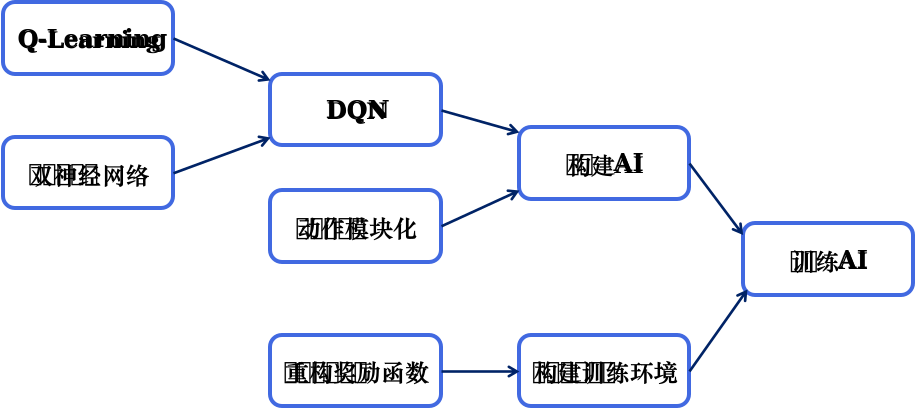
\includegraphics[width=0.5\textwidth]{image//开发流程图.png}} 
	\caption{第二阶段项目开发示意图} \label{} 
\end{figure}

\subsection{DQN算法框架回顾}
在第二阶段,我们使用了Deep Q-learning,也称 Deep Q-network(简称 DQN)
作为强化学习的底层算法。DQN的算法流程如下所示:
\begin{figure}[H]
	\centering
	{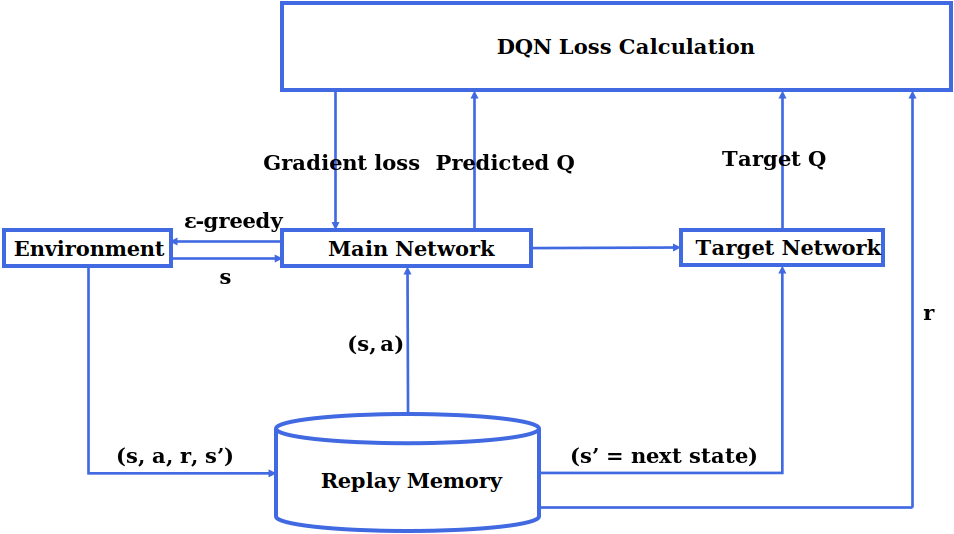
\includegraphics[width=0.5\textwidth]{image//DQN结构.png}} 
	\caption{DQN算法流程图} \label{} 
\end{figure}

从数学原理上看,DQN使用了随机梯度下降的方式,近似求解贝尔曼最优方程
$Q(s,a) = \mathbb{E}\left[ r_{t+1} + \gamma \mathop{\max}_{a\in \mathcal{A}(s_{t+1})} Q_t(s_{t+1},a) \Big| s_t=s,a_t=a \right]$。
从模型特点上看,DQN使用了两个神经网络(main network与target network)异步更新,
并从经验池(replay buffer)中抽取样本进行训练。

DQN技术主要有两个特点:双神经网络与经验回放。第一项技术是使用主网络和目标网络,并进行异步更新。
主网络频繁更新,而目标网络则在短期内保持不变。
在每次迭代中,我们从经验池(replay buffer)中按照均匀分布随机抽样出一批样本 $\{(s_t,a_t,r_t,s_{t+1})\}$
输入主网络。主网络给出估计值$\hat{Q}(s,a;w)$,目标网络给出目标值$r + \gamma \mathop{\max}_{a\in \mathcal{A}(s')}\hat{Q}(s',a;w)$的估计,
然后使用随机梯度下降的方式,最小化损失函数的期望。在一定轮次之后,将主网络的权重覆盖到目标网络上。 

第二项技术是经验回放(experience replay)。当我们收集一些经验样本后,我们不按照收集的顺序来使用它们,
而是将它们储存在回放缓冲区里。每次更新主网络时,我们按照均匀分布从回放缓冲区中提取一组样本(batch)。
尽管样本是贯序收集的,相邻样本之间具有显著的相关性,但是使用抽样的方式,则可以打破样本间的前后相关性,
让神经网络从样本中学习到更普适性的知识。此外,通过将经验保存在经验池中,每个经验都可以被多次学习,
也提高了经验利用率。

\subsection{本阶段创新点汇总}
由于AI无法直接“看到”战场的情况,因此,需要认为提取重要特征并输入神经网络。
在第二阶段,我们基于观察经验,提取了7个有代表性的战场特征,分别是:
\textbf{天然矿石数量、战舰规模、舰队分布、已采矿石、船厂分布、敌方舰队动向、我方舰队动向},
构成$21 \times 21 \times 7$的张量,输入神经网络对$Q(s, a_i)$进行拟合。

在训练AI执行动作时,我们发现,直接让AI学会制定各个船厂的具体指令十分困难。
比如,AI难以学会直接制定出“N10E5C”“N5E6S5W”这类精巧复杂的舰队指令。
于是我们转变了思路,为AI提供一些封装成模块的动作,
将基本动作采用不同顺序组合在一起,组合出了优先进攻、优先挖矿、优先扩张、优先防御、中庸之道共5套“组合拳法”,
让AI根据战场状况,选择最适合的组合动作。

在构建训练训练环境时,我们小组重构了奖励函数,使用了根据战局进程而调整各要素权重的综合评分奖励机制,
并着重考虑了四种要素的价值:已经开采并且运回大本营的矿石、已经开采但仍然由舰队携带的矿石、舰队和船厂。 

在训练的过程中,我们采用$\epsilon$-greedy的策略,随着训练的进行,$\epsilon$从1逐渐下降到0.2,
我们使AI始终保持一定的探索性,防止陷入局部最优解。此外,我们还为AI提供多种不同的对手,并且让AI进行自我对弈,
使AI能够更快提升能力。

\section{第三阶段介绍:更多样的战场特征与更灵活的动作设计}
\subsection{将战场特征扩展到12层}
在本阶段,我们提取了12层的特征,分别是:
\textbf{天然矿石数量、战舰规模、舰队分布、已采矿石、船厂分布、敌方舰队动向、我方舰队动向、
敌方高威胁性船厂、敌方高威胁性舰队、我方无家可归的舰队、敌方无家可归的舰队、敌方试图攻击我方船厂的舰队},
共构成$21\times 21 \times 12$的张量输入神经网络。其中,前7个特征是在上一阶段提取的,
后5个特征是在本阶段提取的。对后5个特征的介绍如下:

\begin{itemize}
	\item  \textbf{敌方高威胁性船厂}:可以简单理解为“建在我家门口的敌军船厂”。如果敌方的某船厂距离我方的某一个船厂的距离
			低于2,则认为是高威胁性船厂,在数组中用$(-1\times shipyard.maxSpawn)$,也即该敌军船厂每回合能制造的船越多,就越危险。
			这个特征是基于本小组在观察第二阶段的战斗历史记录后提出的。
			我们发现,靠近我方的敌军船厂非常容易对我方的船厂进行骚扰,甚至能够较为轻松地攻克。
			但在第二阶段,AI可能会对高威胁性的敌方船厂视而不见,这十分危险。因此我们补充了这个特征。
	\item  \textbf{敌方高威胁性舰队}:可以简单理解为“跑到我家门口的敌军舰队”。如果敌方的某舰队的下一步位置,
			到我方某船厂的距离小于等于1,则认为该敌军舰队是高威胁性的敌军舰队,在数组中用$(-1\times shipCount)$表示,
			也即该敌方舰队规模越大,则越有威胁性。
	\item  \textbf{我方无家可归的舰队}:我们经过观察发现,如果我方的舰队在飞行中途与敌方撞击,损失部分舰队,则可能无法执行
			所有的飞行计划,无法回到船厂,会一直在外面游荡,所采集的矿石无法运回,十分可惜。因此考虑对其进行单独表征,
			并在动作设计时加入拯救该舰队的动作。在数组中用$(+1*shipCount)$表示我方无家可归舰队。
	\item  \textbf{敌方无家可归的舰队}:类似的,我们发现敌方也有可能存在无家可归的舰队,这些舰队所采集的矿石,也可以被我方所“截获”。
			在数组中用$(-1*shipCount)$表示敌方无家可归舰队
	\item  \textbf{敌方试图攻击我方船厂的舰队}:指那些当前未必属于高威胁性(未必在我方船厂附近),但飞行路线上是冲着我方某个船厂而来的敌方舰队。
			这些舰队尽管威胁性较低,但仍然需要警惕,需要提前做好防备和反击。在数组中用$(-1*shipCount)$表示敌方试图攻击我方船厂的舰队。
\end{itemize}


\subsection{将动作“组合拳”扩展到10种}
延续上一阶段的思路,我们为AI提供了更加灵活、多样、精细的模块化动作。
目前一共配备了10套“组合拳”,分别是:
\textbf{优先进攻、优先挖矿、优先扩张、优先防御、中庸之道、优先攻击敌方高威胁船厂、优先防备敌方高威胁性舰队、
带我回家、趁火打劫、群起而攻之}
前五个“组合拳”是上一阶段设计的,后5套组合拳是这本阶段设计的,简要介绍如下:
\begin{itemize}
	\item \textbf{优先攻击敌方高威胁船厂}:寻找敌方所有高威胁性船厂。如果有多个高威胁性船厂,则选取最弱的进行围攻。
			所有距离该高威胁船厂距离小于2的我方船厂,都尽可能地多派出舰队攻击它;
			所有距离大于2而小于等于10的我方船厂,则派出的船队规模随距离递减,从40递减到12;这是因为距离越远,
			则不确定性越大,越不适合进行远距离奔袭攻击。如果对方目前没有高威胁性船厂,则转入保守的防御策略。
	\item \textbf{优先防备敌方高威胁性舰队}:寻找敌方所有高威胁性的舰队,并确定敌方该舰队威胁到的是我方的哪一个船厂。
			如果受威胁的我方船厂拥有的船只数量大于等于敌方舰队,则不用害怕,只需要努力生产船只,抵抗冲击即可。
			如果受威胁的我方船厂的舰队规模小于敌方舰队,则要在坚决抵抗和走为上策之间做出抉择。
			如果我方该船厂的每回合最大舰队生产数量大于4,说明该船厂被我方控制的时间比较久,目前船厂内缺少船只,
			可能是因为都派出去采矿了,等那些舰队采矿回来,仍然有可能可以把这个船厂夺回来,因此该船厂只需要努力生产船只,
			抵抗敌方冲击即可,等待援兵到来。如果我方该船厂的每回合最大舰队生产数量小于等于4,说明该船厂被我方控制时间比较短,
			则考虑放弃这个船厂,将船只全部转移到我方其他船厂。若我方已经没有其他船厂了,则攻击敌方最弱的船厂。
	\item \textbf{带我回家}:也即拯救我方无家可归舰队。若有我方有多个无家可归的舰队,则选取采矿数量最多的舰队,
			因为采矿数量最多,也最值得拯救。我方拥有船只数量最多(实力最雄厚)的船厂,
			会派出一个舰队规模大于该无家可归的舰队,与其合并,并带回我方船厂。
	\item \textbf{趁火打劫}:与“带我回家”相反,“趁火打劫”意在拦截对方无家可归舰队。若敌方有多个无家可归的舰队,则选取采矿数量最多的舰队,
			因为采矿数量最多,也最值得拦截。我方拥有船只数量最多(实力最雄厚)的船厂,
			会派出一个舰队规模大于该无家可归的敌方舰队,与其对撞,并把我方夺得的敌军矿石送回我方船厂。
	\item \textbf{群起而攻之}:围攻敌方最弱的船厂。最弱的定义方式是——找出敌方造船能力最低的2个船厂(也即控制的时间最短),
    			在其中选择拥有船只数量最少的那个船厂作为最弱船厂。选定敌方最弱船厂后,我方各个船厂在自身实例足够雄厚的情况下,
				会各派规模为35的舰队对敌方该最弱船厂进行围攻。
				这个策略可以让防守策略设计得不好的对手难以察觉、无法精准防范。
\end{itemize}


\section{小结:三个阶段的设计理念}
在三个阶段中,本小组一以贯之的设计理念是:\textbf{将人类的先验知识,与人工智能算法相互结合}。
比如第一阶段引入启发式,防止AI出现“短见”行为;第二阶段对奖励函数进行重构,引导AI合理使用挖矿策略。
第三阶段则在基于对第二阶段的对战历史记录的观察上,设计出了防范对方高威胁性船厂、舰队,以及
回收无家可归舰队的策略。我们相信,将人类的经验智慧,与计算机的强大计算能力结合,并不断开发更高效稳健的算法,
是未来人工智能发展的一个十分有潜力的方向。

\section*{附注}
由于第三阶段时间较为匆忙,我们尚未来得及训练第三阶段的AI。我们将第三阶段的训练环境、模块化动作设计一并附上,
以供参考。

\end{document}

% \begin{figure}[H]
% 	\centering
% 	{\includegraphics[width=0.35\textwidth]{image//ignorance.png}} 
% 	\caption{} \label{} 
% \end{figure}


% \lstinputlisting[style = Python,
% caption={Python codes},
% label = {efficient},
% linerange={110-125}]{exercise3.py} 


% \begin{figure}[H]
%     \centering
%     \subfigure[patch size = 11]
%     {\label{} \includegraphics[width=0.49\textwidth]{image//local equalization with patch size = 11.jpg}}
%     \,    
%     \subfigure[patch size = 51]
%     {\label{} \includegraphics[width=0.49\textwidth]{image//local equalization with patch size = 51.jpg}}
%     \,
%     \subfigure[patch size = 151]
%     {\label{} \includegraphics[width=0.49\textwidth]{image//local equalization with patch size = 151.jpg}}
%     \,    
%     \subfigure[patch size = 201]
%     {\label{} \includegraphics[width=0.49\textwidth]{image//local equalization with patch size = 201.jpg}}
%     \caption{local equalization with different patch sizes}\label{} 
% \end{figure}
